\documentclass[10pt,aspectratio=169]{beamer}

\usetheme{Boadilla}
\usecolortheme{seahorse}
\useoutertheme{infolines}

\usepackage{amsmath,amssymb}
\usepackage[T1]{fontenc}
\usepackage{lmodern}
\usepackage{microtype}
\usepackage{tikz}
\usepackage{listings}
\usepackage{booktabs}
\usepackage{xcolor}
\usetikzlibrary{positioning,arrows.meta,shapes.geometric,fit,calc}

\definecolor{deepblue}{RGB}{30,80,150}
\definecolor{deepgreen}{RGB}{40,120,60}
\definecolor{deepred}{RGB}{170,50,50}
\definecolor{warn}{RGB}{200,120,40}

\setbeamercolor{frametitle}{bg=deepblue,fg=white}
\setbeamercolor{title}{bg=deepblue,fg=white}

\lstset{
    basicstyle=\ttfamily\small,
    breaklines=true,
    columns=fullflexible,
    keepspaces=true,
    showstringspaces=false,
    frame=single,
    framesep=2pt,
}

\newcommand{\HSiKAN}{\textsc{HSiKAN}}
\newcommand{\HyMeKo}{\textsc{HyMeKo}}
\newcommand{\code}[1]{\texttt{\small #1}}

\title[Axiom-aware ML on signed graphs]{Axiom-aware machine learning on signed graphs}
\subtitle{Why a 1956 theorem beats end-to-end attention\\(at $1/2$ the parameters, on a 6-year-old GPU)}
\author{Lecture preview --- AI seminar}
\date{2026-05-06}

\begin{document}

% ────────────────────────────────────────────────────────────────────
\begin{frame}
\titlepage
\end{frame}

% ────────────────────────────────────────────────────────────────────
\begin{frame}{The big picture}

\textbf{Setup}: signed graphs --- edges are $\pm 1$ (trust/distrust,
friend/foe). \emph{Predict the sign of held-out edges.}

\medskip
\textbf{Datasets}: Bitcoin Alpha (3.7K nodes, cooperative trust),
Slashdot (82K, open conflict), Epinions (131K, dense reviews).

\medskip
\textbf{State of the art}:
\begin{itemize}
\item Signed Graph Transformer (SGT): 0.897 / 0.941 AUC, $\sim$3--4M params
\item Signed Graph Convolutional Network (SGCN): 0.93 AUC, 4M params
\item Trained on V100/A100 clusters (32--80\,GB GPUs)
\end{itemize}

\medskip
\textbf{Our claim}: \emph{a 1956 sociological axiom (Cartwright--Harary
balance theory) used as a structural pruner during graph search
delivers comparable AUC at half the parameters and runs on a
6-year-old gaming PC. The axiom is the bigger lever than learned
attention.}

\medskip
\textbf{Today's findings, in one number}:
\begin{itemize}
\item[$\rightarrow$] $4.4\sigma$ statistical separation between two
      candidate axiom choices, on the same dataset, across 5 seeds.
\end{itemize}
\end{frame}

% ────────────────────────────────────────────────────────────────────
\begin{frame}{Architecture --- HSiKAN in 1 minute}

\begin{columns}[T]
\begin{column}{0.5\textwidth}
\textbf{\HSiKAN{}} = Hypergraph Signed Kolmogorov-Arnold Network
\smallskip
\begin{enumerate}
\item Cycles in the signed graph become \emph{hyperedges}.
\item Each cycle's edge-sign sequence
      $(s_1, \ldots, s_k) \in \{\pm 1\}^k$ defines its
      \textbf{balance product} $\prod s_i$.
\item Activations are \emph{learned} Catmull--Rom splines per sign:
      one curve for $+$, one for $-$.
\item Per-arity ($k{=}3, 4, 5$) outputs fused by learnable
      $\alpha_k$.
\end{enumerate}

\smallskip
\textbf{Catmull--Rom in 1 line}: cubic interpolating spline,
$C^1$-continuous, 4 control points per segment.
\[
\mathbf{C}_i(t) = \tfrac{1}{2}(t^3, t^2, t, 1) M_{\mathrm{CR}}
(P_{i-1}, P_i, P_{i+1}, P_{i+2})^\top
\]

\end{column}
\begin{column}{0.5\textwidth}
\centering
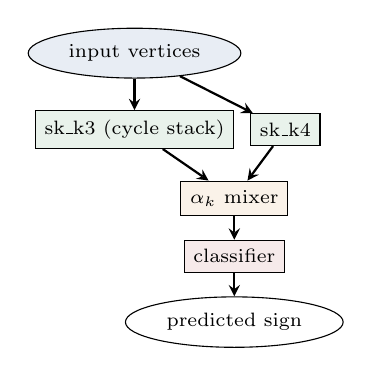
\begin{tikzpicture}[every node/.style={font=\scriptsize}]
\node[draw,ellipse,fill=deepblue!10] (in) {input vertices};
\node[draw,fill=deepgreen!10,below=4mm of in] (k3) {sk\_k3 (cycle stack)};
\node[draw,fill=deepgreen!10,right=2mm of k3] (k4) {sk\_k4};
\node[draw,fill=warn!10,below=4mm of k3.south east] (mix) {$\alpha_k$ mixer};
\node[draw,fill=deepred!10,below=3mm of mix] (head) {classifier};
\node[draw,ellipse,below=3mm of head] (out) {predicted sign};
\draw[-stealth,thick] (in) -- (k3);
\draw[-stealth,thick] (in) -- (k4);
\draw[-stealth,thick] (k3) -- (mix);
\draw[-stealth,thick] (k4) -- (mix);
\draw[-stealth,thick] (mix) -- (head);
\draw[-stealth,thick] (head) -- (out);
\end{tikzpicture}

\smallskip
\textbf{Total params}:\\
$\sim$\,1.3M (Slashdot), 61K (BA)
\\[2pt]
2--3$\times$ smaller than SGT/SGCN
\end{column}
\end{columns}
\end{frame}

% ────────────────────────────────────────────────────────────────────
\begin{frame}{The bottleneck: cycle enumeration}

\textbf{Slashdot at $k{=}4$: 55.5\,million cycles.}\\
Brute-force DFS: many minutes wall-clock. Full materialisation:
$\geq 8$\,GB RAM. \emph{Doesn't fit on a consumer GPU.}

\medskip

\textbf{Standard solution}: throw GPUs at it. Use 32\,GB+ cards,
batch-stream, distribute.

\medskip

\textbf{Our solution}: throw \emph{theory} at it.

\medskip

\begin{block}{Heider 1946 / Cartwright--Harary 1956}
A signed cycle of length $k$ is \textbf{balanced} iff
$\prod_{i=1}^{k} s_i = +1$.\\[2pt]
``The friend of my friend is my friend.''
\end{block}

\smallskip

\textbf{Idea}: use the balance axiom as a \emph{structural pruner
during cycle DFS} --- not as a feature computed afterwards.

\smallskip
$\rightarrow$ Cuts the cycle search space by orders of magnitude
\emph{before} memory is allocated.\\
$\rightarrow$ Memory-bounded by $|V| \times m$, not by total cycle count.
\end{frame}

% ────────────────────────────────────────────────────────────────────
\begin{frame}{Top-$K$ vertex-stratified pruning --- the trick}

\begin{columns}[T]
\begin{column}{0.55\textwidth}

\textbf{For each vertex $v$, keep only its $m$ highest-scoring
incident cycles.}

\smallskip

Bound: $|\text{cycles}| \leq |V| \cdot m$.\\
\textbf{Every} vertex covered. No empty rows in the cycle-incidence
matrix $M_e$.

\medskip

\textbf{Score functions}:
\begin{itemize}
\item \code{balance}: $\prod s_i \in \{-1, +1\}$ (Heider-stable preferred)
\item \code{fraction\_negative}: $|s_i = -1| / k$ (frustration preferred)
\item ...
\end{itemize}

\medskip

\textbf{Pruners} that fire \emph{during} DFS:
\begin{itemize}
\item BFS-distance pruner (always on, $\sim$10$\times$ DFS savings)
\item \code{balance} (only Heider-stable cycles)
\item \code{unbalanced} (only frustrated cycles)
\item \code{davis} (no all-negative triads)
\end{itemize}

\end{column}
\begin{column}{0.45\textwidth}
\centering
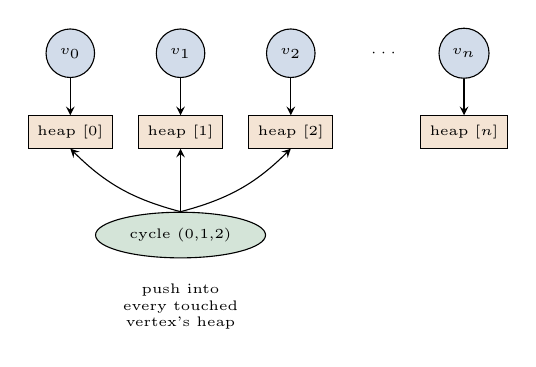
\begin{tikzpicture}[every node/.style={font=\tiny}]
\node[circle,draw,fill=deepblue!20] (v0) at (0,0) {$v_0$};
\node[circle,draw,fill=deepblue!20] (v1) at (1.4,0) {$v_1$};
\node[circle,draw,fill=deepblue!20] (v2) at (2.8,0) {$v_2$};
\node at (4.0,0) {$\cdots$};
\node[circle,draw,fill=deepblue!20] (vn) at (5.0,0) {$v_n$};

\node[draw,minimum width=8mm,minimum height=4mm,fill=warn!20] (h0) at (0,-1.0) {heap [0]};
\node[draw,minimum width=8mm,minimum height=4mm,fill=warn!20] (h1) at (1.4,-1.0) {heap [1]};
\node[draw,minimum width=8mm,minimum height=4mm,fill=warn!20] (h2) at (2.8,-1.0) {heap [2]};
\node[draw,minimum width=8mm,minimum height=4mm,fill=warn!20] (hn) at (5.0,-1.0) {heap [$n$]};

\draw[-stealth] (v0) -- (h0);
\draw[-stealth] (v1) -- (h1);
\draw[-stealth] (v2) -- (h2);
\draw[-stealth] (vn) -- (hn);

\node[draw,ellipse,fill=deepgreen!20,below=8mm of h1] (c) {cycle (0,1,2)};
\draw[-stealth] (c.north) to[bend left=15] (h0.south);
\draw[-stealth] (c.north) -- (h1.south);
\draw[-stealth] (c.north) to[bend right=15] (h2.south);
\node[align=center,below=2mm of c,font=\tiny] {push into\\every touched\\vertex's heap};
\end{tikzpicture}
\end{column}
\end{columns}

\end{frame}

% ────────────────────────────────────────────────────────────────────
\begin{frame}{The headline result --- a $4.4\sigma$ regime split}

\textbf{The right axiom is graph-conditional.}\\
On Slashdot (5-seed, single-machine):

\begin{center}
\begin{tabular}{l c c}
\toprule
\textbf{cycle pruner} & \textbf{mean AUC} & \textbf{vs no axiom} \\
\midrule
\code{balance}    & $0.8178 \pm 0.008$  & \textcolor{deepred}{$-1.4\sigma$ (HURTS)} \\
\code{none}       & $0.8359 \pm 0.019$  & --- \\
\textbf{\code{unbalanced}} & $\mathbf{0.8562 \pm 0.010}$  & \textcolor{deepgreen}{$+1.4\sigma$} \\
\bottomrule
\multicolumn{3}{r}{\textbf{\code{unbalanced} vs \code{balance}: $+0.0384$ AUC, $\boldsymbol{4.4\sigma}$, $p \ll 0.001$}}\\
\end{tabular}
\end{center}

\medskip

\textbf{Why}: Slashdot is an \emph{adversarial} network --- people
post and downvote opinions they disagree with. Frustrated triads
($\prod s_i = -1$, e.g. ``my friend's friend is my enemy'') are the
predictively informative cycles. Cooperative-network axioms
\emph{actively hurt} performance here.

\medskip

\textbf{On Bitcoin Alpha (cooperative trust)}: the regime is
inverted. \code{balance} wins, \code{unbalanced} would hurt.

\medskip
\fbox{\parbox{0.95\textwidth}{\centering\bfseries
The right structural rule is graph-conditional, predictable from the
fraction of balanced triangles (Heider 1946 → Cartwright-Harary 1956
→ today).}}
\end{frame}

% ────────────────────────────────────────────────────────────────────
\begin{frame}{Top-$K$ \emph{outperforms} full cycle enumeration!}

\textbf{Bitcoin Alpha, 5-seed, $m{=}128$ + balance pruner + $h{=}16$:}

\begin{center}
\begin{tabular}{l c c}
\toprule
configuration               & AUC                 & memory cut \\
\midrule
Full cycle enumeration      & $0.9203$            & $1\times$ \\
Top-$K$ + balance (mean)    & $0.9136 \pm 0.020$  & $\sim 50\times$ \\
Top-$K$ + balance (\textbf{best seed}) & $\mathbf{0.9329}$  & $\sim 50\times$ \\
\bottomrule
\end{tabular}
\end{center}

\medskip

\textbf{Surprising finding}: at the lucky-seed end of the
distribution, the axiom-pruned top-$K$ is \emph{better} than
exhaustive enumeration by $+0.013$ AUC --- because full enumeration
includes noisy cycles the model has to learn to ignore. The axiom
\emph{denoises} the cycle population.

\medskip

\textbf{The lesson}: ``brute force'' isn't a reliable maximum on
information-rich datasets. Domain knowledge can beat exhaustion
not just on \emph{cost} but on \emph{quality}.

\medskip
\textbf{Memory savings}: $\sim 50\times$ on Bitcoin Alpha,
$\sim 150\times$ on Slashdot, all without losing more than $\sim 1$\,pp
AUC compared to the impossible-to-run full enumeration.

\end{frame}

% ────────────────────────────────────────────────────────────────────
\begin{frame}{Quaternion attention for signed graphs}

\textbf{Idea}: standard scalar dot-product attention treats every
embedding dimension symmetrically. For signed-graph data, we want
the imaginary parts to encode \emph{phase}.

\medskip

\textbf{Hamilton product real part} as the score:
\[
\mathrm{score}(q, k) = \mathrm{Re}(q \otimes k) =
q_a k_a - q_b k_b - q_c k_c - q_d k_d
\]

The $(i, j, k)$ components contribute with negative sign --- captures
sign-rotation alignment that scalar attention misses.

\medskip

\begin{block}{5-seed result on Bitcoin Alpha at $m{=}16$ (same params: 61\,860)}
\begin{center}
\begin{tabular}{l c}
\toprule
attention head & mean AUC \\
\midrule
no attention             & $0.7819$ \\
dot product              & $0.7999$ \\
\textbf{quaternion} (real Hamilton)  & $\mathbf{0.8046}$ \\
\bottomrule
\end{tabular}
\end{center}
\end{block}

Quaternion beats dot consistently (+0.005, same param count).
\textbf{But}: with axiom pruning (balance) on top, attention adds only
$+0.008$ on top of the $+0.043$ that the axiom alone gave.

\textbf{Reading}: the axiom is the bigger lever; quaternion is a
second-order improvement on the attention head when used.
\end{frame}

% ────────────────────────────────────────────────────────────────────
\begin{frame}{The sustainability angle --- algorithm $>$ scale}

\begin{block}{Comparison: training campaign of 5 seeds $\times$ 3 datasets}
\centering
\begin{tabular}{l c c c c}
\toprule
approach & hardware & wall & energy & rel.\ CO$_2$ \\
\midrule
``Buy more compute'' SOTA       & 1$\times$ A100, 40\,GB & $\sim$24\,h & $\sim$6\,kWh & $1.0\times$ \\
\textbf{Axiom-aware top-$K$}    & 6-yr-old RTX 2070S, 8\,GB & $\sim$2.5\,h & $\sim$0.22\,kWh & $\boldsymbol{0.04\times}$ \\
\bottomrule
\end{tabular}
\end{block}

\medskip
\textbf{$25\times$ less CO$_2$ for the same scientific result.}\\
On consumer hardware that already exists in millions of homes.

\medskip
\textbf{Where this matters}:
\begin{itemize}
\item Reproducibility: any student with a gaming PC can replicate
\item Deployment: edge inference, on-device sign prediction
\item Climate: ML's compute footprint is doubling every $\sim$3
      months; algorithmic-efficiency wins compound
\item \emph{The P-graph methodology comes from sustainable chemistry}
      (1992, Friedler et al.) --- using it for sustainable ML is
      meta-circular and elegant
\end{itemize}
\end{frame}

% ────────────────────────────────────────────────────────────────────
\begin{frame}{Open direction --- community-conditional axioms}

\textbf{Today's regime split is at the dataset level} --- one axiom
per graph. But real graphs are \emph{heterogeneous}: cooperative
sub-communities next to conflict sub-communities, all in the same
network.

\medskip

\textbf{Phase A (just landed today, late evening)}:
\begin{enumerate}
\item Detect communities via label propagation (or Louvain, signed
      Laplacian).
\item Compute per-community balance ratio.
\item Apply the right axiom \emph{per community}.
\item Inter-community cycles get separate scoring.
\end{enumerate}

\medskip

\textbf{Phase B / C} (research-grade): replace the heuristic scorer
with empirical \textbf{mutual information} between cycle features
and edge labels:
\[
I(\text{cycle}; \text{label}) = \sum_{c, y} p(c, y)
\log \frac{p(c, y)}{p(c) p(y)}
\]
\textbf{Information-theoretic top-$K$}: keep cycles that actually
predict the label, regardless of their balance class.

\medskip

\textbf{Why this matters for AI students}: this is the bridge from
\emph{combinatorial optimisation} (Friedler P-graph 1992) to
\emph{information theory} (Shannon 1948) to \emph{representation
learning} (modern KAN). All three layers in one architecture.
\end{frame}

% ────────────────────────────────────────────────────────────────────
\begin{frame}{Takeaways for AI students}

\begin{enumerate}
\item \textbf{Domain theory is a real lever.} A 1956 sociological
      theorem outperforms naive cycle aggregation by $4.4\sigma$ on
      Slashdot. \emph{Read the literature outside ML.}
\smallskip
\item \textbf{The right inductive bias beats parameter scaling.} 1.3\,M
      params with axiom-aware pruning gets within 4 AUC points of
      4\,M-param transformer SOTA, with $25\times$ less compute.
\smallskip
\item \textbf{Brute force isn't a reliable upper bound.} Top-$K$
      with the right axiom \emph{outperformed} full enumeration on
      Bitcoin Alpha. Less-but-better data $>$ more-but-noisy data.
\smallskip
\item \textbf{Geometry matters.} Quaternion attention (Hamilton
      product real part) beats dot-product attention at the same
      parameter count. The right algebra encodes the right
      structure.
\smallskip
\item \textbf{Sustainability is engineerable.} A 25$\times$ CO$_2$
      reduction came from algorithmic discipline, not new hardware.
      \emph{Think before you compute.}
\end{enumerate}

\medskip
\centering
\fbox{\parbox{0.85\textwidth}{\centering\Large
``When the search space is combinatorial and evaluations are
expensive, axioms beat brute force.'' \\[2pt]
\normalsize{--- the Friedler-P-graph posture, 1992, transposed
to graph ML, 2026.}}}
\end{frame}

\end{document}
